\chapter{Dataset Suitability for Melanoma Detection}

\section{Introduction}
This chapter contains an analysis of some popular datasets including ISIC 2019, and PH2. The goal is to identify any relationships between skin lesions and patients. Using this analysis `the dataset' is created using NHS macroscopic images and metadata.

There is an analysis of the distribution of metadata in these datasets, discussing whether they are consistent with the literature. For example, SK is more likely to have milia-like cysts compared to melanoma. So we check if the distribution of data in datasets specifies this. The reasoning for this is that a Bayesian network is used later and trained on datasets based on the distribution of data. Therefore ensuring that the data is scientifically relevant ensures the Bayesian network is functioning correctly. Certain criteria are found to be ineffective and removed because they are not consistent with the literature.

\section{Other Datasets}
The analysis of skin lesions is an especially laboured field, so there are a huge number of relevant datasets to discuss. Public datasets include MEDLINE, PH2, ISIC, and others making a total of 21 open-access datasets containing 106,950 skin lesion images\cite{Wen2022}. Out of these datasets, only the PH2 dataset has publicly accessible metadata regarding ABCD rules with a total of 200 images. ISIC is the largest of these datasets, being a combination of many other datasets, with extra annotations from the original.

%Go into more detail and graphs
\begin{table}
	\small
	\begin{tabular}{|c|c|p{0.15\linewidth}|c|c|p{0.34\linewidth}|}
		\hline
		Name             & Year & Image Type                 & Number & Classes & Metadata                                                                                                 \\
		\hline
		ISIC 2019        & 2019 & Dermoscopic                & 33,569 & 8       & Age, anatomical site, gender, and diagnosis
		\\
		\hline
		PH2              & 2013 & Dermoscopic                & 200    & 3       & Asymmetry, colour, pigment network, dots/globules, streaks, regression areas, blue-whitish veil
		\\
		\hline
		MED-NODE         & 2015 & Macroscopic                & 170    & 2       & n/a
		\\
		\hline
		SD-198           & 2016 & Dermoscopic \& Macroscopic & 6,584  & 198     & anatomical site, symptoms, duration, morphology, and colour
		\\
		\hline
		SKINL2           & 2019 & Macroscopic (unique tool)  & 376    & 8       & Gender, age, and fototype
		\\
		\hline
		7-point Criteria & 2018 & Dermoscopic \& Macroscopic & 2000   & 2       & Pigment network, regression, pigmentation, blue-whitish veil vascular structures, streaks, dots/globules
		\\
		\hline
	\end{tabular}
	\caption{}
\end{table}\label{datasets}

The datasets listed in table\ref{datasets} include the number of images, classes, and metadata. Out of these datasets ISIC 2019, PH2 and 7-Point Criteria appear to be the most promising. PH2 is especially useful because it is the only dataset representing ABCD rules on asymmetry and colour. SKINL2 was considered, but ISIC 2019 was a much larger dataset with more metadata. SD-198 is publicly available but not accessible.

Overall ISIC 2019 and PH2 are the most suitable datasets. The PH2 dataset is utilised for an analysis of feature extraction techniques such as the detection of ABCD rules and dermoscopic structures. Then the entire technique is analysed using the ISIC 2019 dataset, which is the largest public dataset.

\section{Issues}
One fundamental problem is the overutilisation of private or privately annotated datasets, making a direct comparison of algorithms (especially relating to ABCD rules) difficult. Some are between benign and malignant\cite{Meskini2018, Kasmi2016, Ali2020b, Ali2020a} while others utilise private or never mention any datasets\cite{Kasmi2016, She2007, Tenenhaus2010, Ramezani2014, Zaqout2016}. None compare their ABCD rules, likely because of subjectivity depending on the dermatologists that labelled them. Ideally, more datasets and labels should be public to assess individual rules and reach objective measurements. Until then, testing algorithms conform with malignant, suspicious, or benign. This is espeically true for the PH2 dataset, although it was around before some of these publications it was not used for testing.

Although there is an ISIC 2020 dataset with a total of 44,108 images, its diagnosis is between benign and malignant and other metadata is on atypical melanocytic proliferation, café au lait macule, lentigo NOS, lichenoid keratosis, naevus, seborrhoeic keratosis, solar lentigo, and other/unknown. The metadata is very specific and doesn't match the requirements of the project, so ISIC 2019 is still a better candidate.

\subsection{ISIC}
The ISIC dataset is a collaborative effort of many institutions to support the development of automatic classification methods for melanoma detection. The most recent applicable dataset is ISIC 2019, which contains a total of 25,331 images for training and 8,238 for testing, making 33,569 images in total. Each image has corresponding metadata including sex, age, anatomical site, and diagnosis. These images are separated into classes melanoma (MM), melanocytic nevus (MV), basal cell carcinoma (BCC), actinic keratosis (AC), benign keratosis (BC), dermatofibroma (DF), vascular lesions (VL), and squamous cell carcinoma (SCC). This includes segmentation masks.

%Show images in the ISIC dataset showing how some of them are different
\begin{figure}
	\centering
	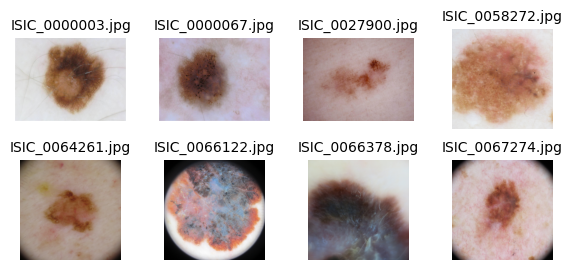
\includegraphics[scale=0.75]{images/ISIC/isic-example-images.png}
	\caption{Examples from the ISIC 2019 dataset, where first two images are BN, followed by two SK, and four MM.}
\end{figure}\label{isic-example-images}

Images in the dataset shown in figure\ref{isic-example-images} are captured with a dermoscope and making it substantial for analysing the structures of the skin lesion. However, many of the lesions have incomplete borders, which is especially true for MM because of its increased size to other lesions. It would be a good idea to detect and remove samples that do not have a complete border when analysing ABCD rules.

%Graph showing one of each type of diagnosis
\begin{table}
	\small
	\begin{tabular}{|c|c|c|c|c|}
		\hline
		Name      & Year       & Total Samples & Differences                                           \\
		\hline
		HAM10000  & 2018       & 11,526        & n/a
		\\
		\hline
		BCN 20000 & 2016       & 19,424        & Includes nails and mucosa
		\\
		\hline
		MSK       & 2015, 2017 & 3918          & Coloured stickers covering un-applicable skin lesions
		\\
		\hline
	\end{tabular}
	\caption{}
\end{table}\label{ISIC_AF}

%Show stickers, nails, etc as proof

ISIC 2019 is a combined source of data from different hospital datasets including HAM10000, BCN 20000, and MSK described in more detail in table\ref{ISIC_AF}. This is important to mention because each dataset has images captured with differing diagnostic procedures resulting in varying resolutions and styles in which the images are taken. MSK includes coloured stickers covering un-applicable skin lesions that are within the area of the image and the camera appears to be further away. BCN 20000 contains rarer types of images including nails and mucosa, which do not appear in the other datasets. HAM10000 does not appear to have any notable differences, but it is still captured with different tools and resolutions.

%Diagram of the number of images assigned to which diagnoses
\begin{figure}
	\centering
	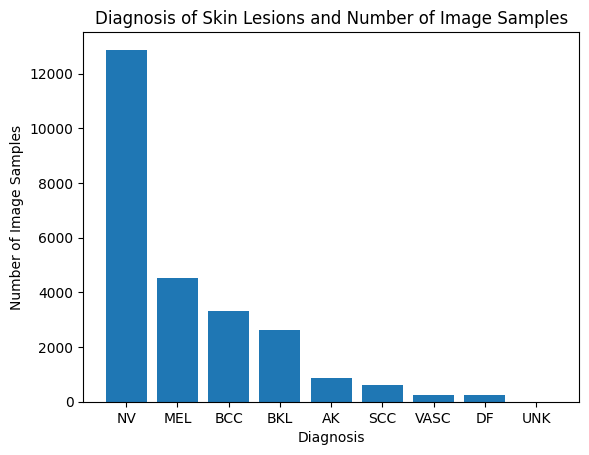
\includegraphics[scale=0.75]{images/ISIC/diagnosis-number.png}
	\caption{ISIC 2019 dataset showing the number of image samples and the diagnosis of those skin lesions dataset appears to be highly unbalanced with half being NV.}
\end{figure}\label{diagnosis-number}

As demonstrated in figure\ref{diagnosis-number} the dataset is highly in-balanced based on the diagnosis of the skin lesion with 12,875 NV and 4,522 MEL. There are only 867 AK, where AK has a very high variance compared to other skin lesions and the sample size is unlikely for adequate detection. Seborrhoeic keratosis (SK) is not in this dataset and AK a similar lesion is described instead. There are only a handful of images for DF, and VASC. The difference in image samples makes the dataset primarily useful for testing between NV and MEL.

\subsubsection{Metdata}
In this dataset, the images are accompanied by metadata describing patient information. This includes patients age, sex, and anatomical location. Analysing this data provides further insight into the influence of patient information on the classification process. Most of all we are looking for similar numbers for each category and some cases might be removed to balance the dataset and improve classification results.

\begin{figure}
	\centering
	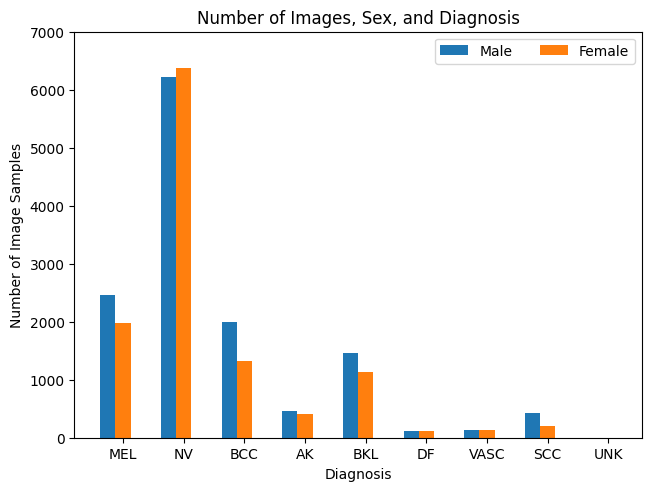
\includegraphics[scale=0.75]{images/ISIC/number-sex-diagnosis.png}
	\caption{The dataset has more male than female patients except for NV which has more samples.}
\end{figure} \label{sex}

Figure\ref{sex} demonstrates the number of samples relating to the patient's sex. There are more samples for each type of skin lesion except for NV which there are slightly more female samples. They are all within a very close range and are unlikely to need rebalancing.

\begin{figure}
	\centering
	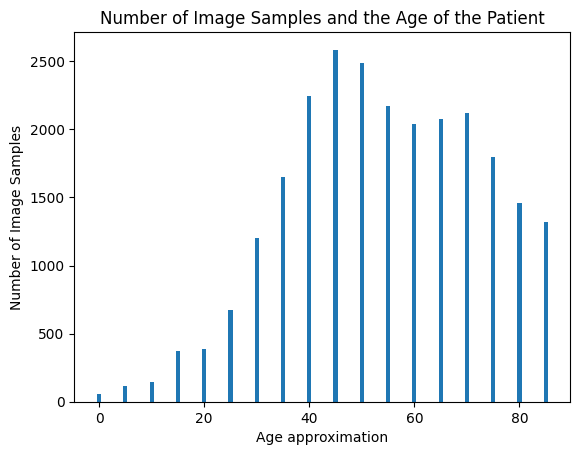
\includegraphics[scale=0.75]{images/ISIC/age-number.png}
	\caption{This shows the number of image samples compared to the age, the dataset is largely unbalanced regarding age where patients are between 40 and 75 years of age.}
\end{figure} \label{age-number}

As demonstrated in figure\ref{age-number} the dataset is unbalanced relating to age and type of skin lesion. Variation is likely a result of skin lesions being more likely to develop in older people than younger ones. This might mean that many of the skin lesions are developed and there is going to be unlikely to find underdeveloped skin lesion samples.

\begin{figure}
	\centering
	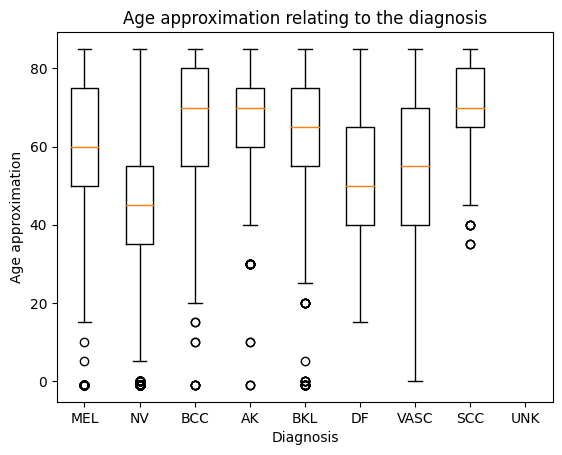
\includegraphics[scale=0.75]{images/ISIC/diagnosis-age.png}
	\caption{The approximate age range of patients and their diagnosis.}
\end{figure} \label{diagnosis-age}

In figure\ref{diagnosis-age} the age approximation (in intervals of 5) was compared with the diagnosis. The black line (whisker) represents the minimum and maximum range of age, the box (quartile) shows the interquartile range (IQR), and the centre line in the middle represents the median. Some dots represent outliers in the data, that are outside the age range.

Each class in the diagram is a diagnosis associated with the age of each patient. Interestingly, represented in this data SCC, BCC, and AK appear to develop more in older adults with a median of age 70. Many younger patients were diagnosed with NV with a median age of 46. Whilst MM appears to be diagnosed in adults with a median age of 60. This is correct when regarding literature\cite{}.


%Consider changing this to a heat map of diagnosis and anatomical location, showing roughly where certain types of skin lesions usually appear

\begin{figure}
	\centering
	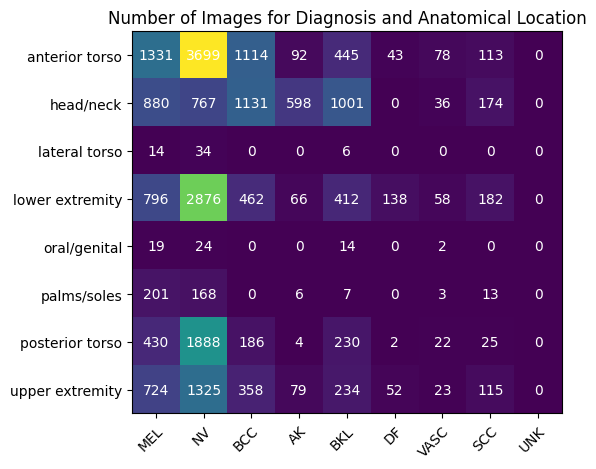
\includegraphics[scale=0.75]{images/ISIC/isic-location-diagnosis.png}
	\caption{Shows image examples associated with the anatomical location and age of the patients.}
\end{figure}\label{isic-location-diagnosis}

The comparison between diagnosis and anatomical location provides further insight into the variety of samples. Figure\ref{isic-location-diagnosis} demonstrates the percentage of image samples (based on the diagnosis) there are for diagnosis and anatomical location. Interestingly, AK appears on 69\% of images on the head/neck. So there is a strong likelihood that skin lesions are overlapping facial features. Furthermore, DF appears more on the lower extremity and upper extremity at 58\% and 22\% respectively. Both AK and DF are consistent with the literature\cite{}.

Another interesting finding is that most skin lesions are in areas of the body that are frequently exposed to the sun, being anterior torso, head/neck, and lower extremities.

\begin{figure}
	\centering
	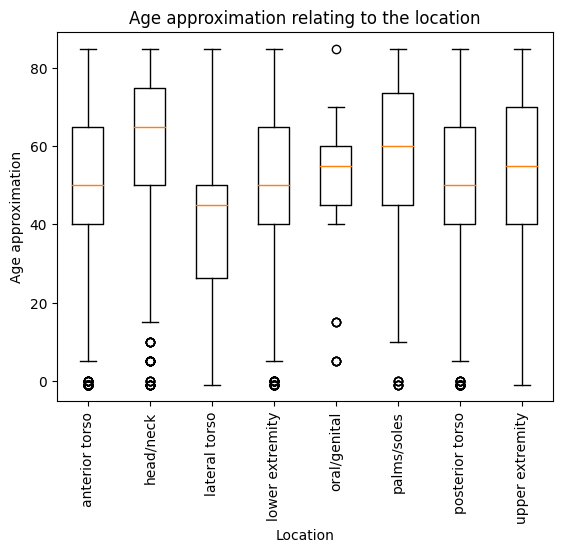
\includegraphics[scale=0.75]{images/ISIC/location-age.png}
	\caption{Shows image examples associated with the anatomical location and age of the patients.}
\end{figure}\label{location-age}

Figure\ref{location-age} is similar to\ref{diagnosis-age}, except it compares the approximate age and location of the skin lesion. There are more older patients who have been diagnosed with skin lesions on their head/neck and younger for the lateral torso. It is concerning that there is a distinct lack of younger patients for palms/soles and head/neck, which could mean more developed skin lesions in these criteria.

\subsubsection{Dermoscopic Structures}
ISIC 2017 shares some images with ISIC 2018 including some additional metadata relating to dermoscopic structure. This includes 2,694 segmentation masks of pigment networks, negative networks, globules, milia-like cysts, and streaks. While the original in ISIC 2017 only has metadata for dermoscopic structures, it was linked to ISIC 2018 using image file names to get their diagnosis. The diagnosis is only between benign naevi, seborrheic keratosis, and melanoma.

\begin{figure}
	\centering
	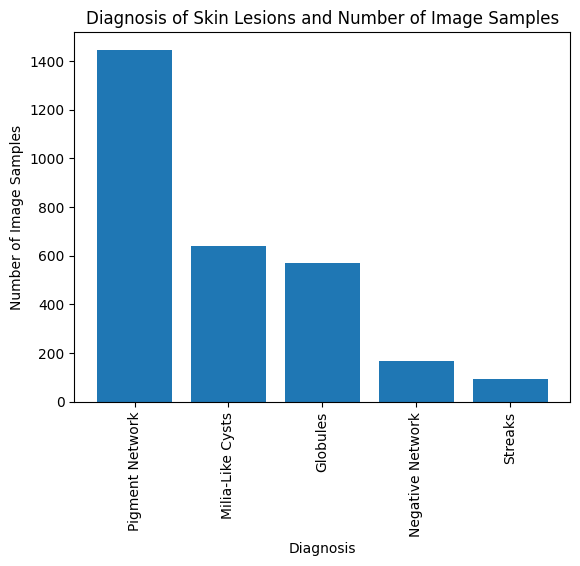
\includegraphics[scale=0.75]{images/ISIC/isic-dermo-number.png}
	\caption{Number of images containing dermoscopic structures.}
\end{figure}\label{isic-number-dermo}

The dermoscopic structures described in figure\ref{isic-number-dermo} show the number of image samples for each dermoscopic structure. Naturally pigmented networks have more than 1400 images which makes it ideal for training a SegNet algorithm. Other dermoscopic structures are lacking, such as streaks has less than 100 images. This is too small for most machine learning algorithms.

\begin{figure}
	\centering
	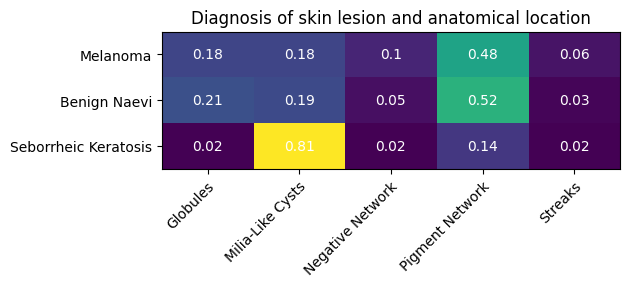
\includegraphics[scale=0.75]{images/ISIC/isic-dermo-diagnosis-heat.png}
	\caption{Number of dermoscopic structures relating}
\end{figure}\label{isic-dermo-diagnosis}

As described in figure\ref{isic-dermo-diagnosis} certain dermoscopic structures are split almost evenly between melanoma and benign naevi, except for streaks and negative networks being more common. This demonstrates the importance of being able to detect the difference between typical and atypical pigmented networks. Furthermore, milia-like cysts appear more frequently in seborrhoeic keratosis and there is a lack of pigmented networks. These are again consistent with the literature.

\subsection{Image Assessment}
The ISIC 2018 dataset is the latest out of the ISIC datasets to have segmentation masks. One of the issues with the segmentation masks is the use of expert and approximate borders that are mixed. There


\subsubsection{Summary}
In summary, the ISIC dataset including data from 2017, 2018, and 2019 makes this dataset the largest public dataset for skin lesion analysis and melanoma detection. It contains a large collection of dermoscopic images with 8 different diagnoses. The dataset having 33,569 makes it ideal for a diverse range of research and development purposes including the evaluation of machine learning and deep learning models. It also contains 2694 images of dermoscopic structures labelled in the ISIC 2017 version of the dataset. Overall, this is the best dataset currently publicly available for the analysis of skin lesions.

Furthermore, data distribution comparing diagnosis to the age, anatomical location, and dermoscopic structures appears to be consistent with literature\cite{}, likely due to the size of the dataset. Otherwise, some image samples have incomplete borders. So, some images should be detected and removed to properly utilise asymmetry, border, and colour.

\subsection{PH2}
The PH2 dataset is a collection of dermoscopic images that were made available in 2013 by Mendonca, et al\cite{}. It consists of 200 images including 80 common nevus, 80 atypical nevus, and 40 Melanoma. Although the dataset is small it holds substantial metadata for describing features within the skin lesion, including asymmetry, colour, pigment network, dots/globules, streaks, regression areas, and blue-whitish veil. This is the only dataset that has such substantial data regarding the mentioned features. Each image has a segmentation mask of the skin lesion.

%Show example images of the PH2 dataset, showing that lots of the melanoma images overlap

\begin{figure}
	\centering
	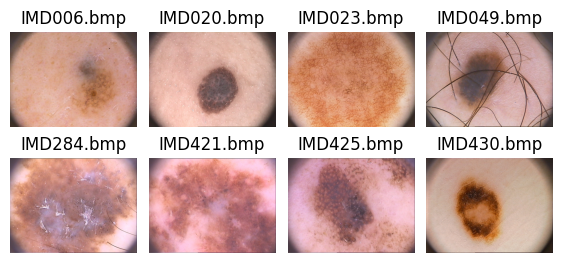
\includegraphics[scale=0.75]{images/ph2/ph2-example-images.png}
	\caption{Example of images from the PH2 dataset. The first two are standard, the second two are atypical, and the last 4 are melanoma.}
\end{figure}\label{ph2-example-images}

The images in figure{ph2-example-images} are some examples of skin lesions from the PH2 dataset. All the images have a circular border and melanoma samples are too big to fit inside the area of the dermoscope in many cases. This results in an incomplete border making it difficult to analyse asymmetry and border from ABCD rules.

\begin{figure}
	\centering
	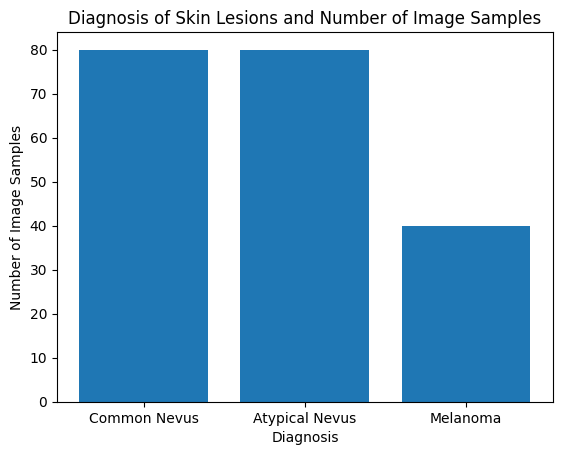
\includegraphics[scale=0.75]{images/ph2/ph2-diagnosis-number.png}
	\caption{Number of image samples and diagnosis in the PH2 dataset.}
\end{figure}\label{ph2-diagnosis-number}

As shown in figure\ref{ph2-diagnosis-number} there are 200 image samples in total with 80 common nevus, 80 atypical and 40 melanoma. The number of image samples is too small for most neural network techniques. The dataset is highly unbalanced with only 40 melanoma images and 160 naevus images. With such a skewed distribution of classes, the model might become overly biased towards the majority class (naevus), leading to poor performance in identifying melanoma. Another issue is the size of these classes, the scarcity of samples will likely result in overfitting when training models. For this reason, this is not a reliable candidate for training machine learning algorithms when considering that more diverse candidates such as ISIC exist.

\subsubsection{Metadata}
The benefit of this dataset is the rich metadata allowing for the analysis of specific features within an image and the relationship between them. This allows for the development of more sophisticated algorithms that provide further insight into the characteristics of melanoma and naevus.

\begin{figure}
	\centering
	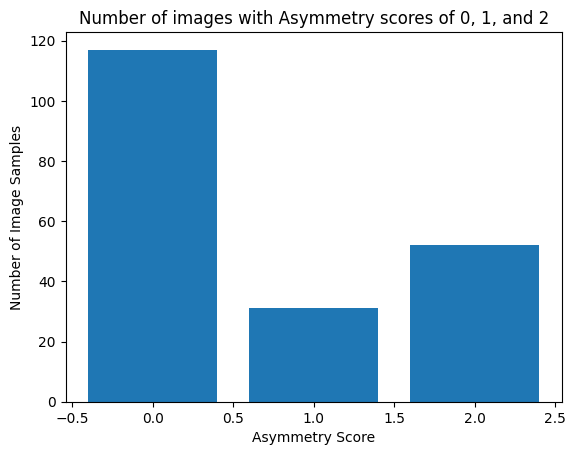
\includegraphics[scale=0.75]{images/ph2/ph2-asym-number.png}
	\caption{This shows the number of image samples and asymmetry score based on Total dermoscopy score (TDS).}
\end{figure}\label{ph2-asym-number}

Demonstrated in figure\ref{ph2-asym-number} demonstrates there is substantial data for measuring the asymmetry score based on the total dermoscopy score (TDS). Typically the algorithms used to measure asymmetry such as bi-fold do not require any training, making the smaller sample size ideal. However, there is a very small sample size for both TDS of 1 and 2, and it would be beneficial to have more.

\begin{figure}
	\centering
	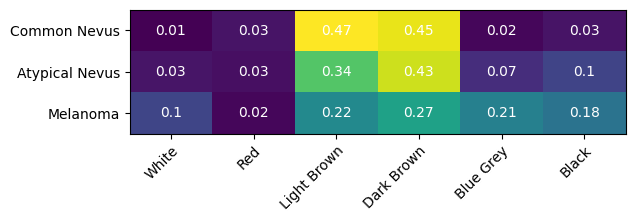
\includegraphics[scale=0.75]{images/ph2/ph2-colour-number-heat.png}
	\caption{Number of colours in the PH2 dataset compared with the diagnosis. Colours are in order white, red, light brown, dark brown, blue-gray, and black.}
\end{figure}\label{ph2-colour-number}

The observation in figure\ref{ph2-colour-number} shows the percentage of images associated with each colour. Light and dark brown are commonly associated with typical naevus. On the other hand, white, blue, and black are more common in melanoma and indicate structural and vascular irregularities. This is true in literature where melanoma is more likely to have a range of colours. The scarcity of red samples demonstrates that it is uncommon in nevus and melanoma. Red is certainly more common in melanoma, but with only a sample size of only 9. The data is likely too stunted to demonstrate this. Other lesions including BCC are more likely to contain red\cite{}, but these lesions are not included in this dataset.

\begin{figure}
	\centering
	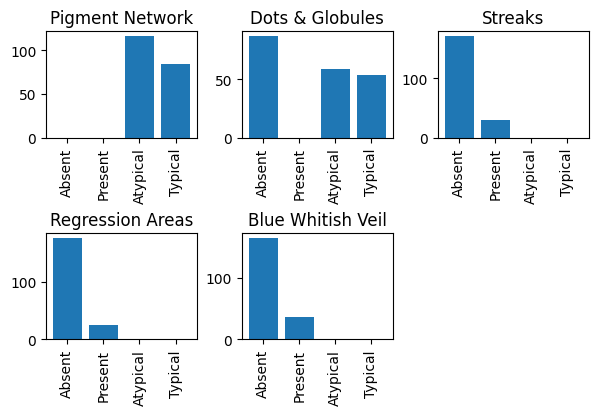
\includegraphics[scale=0.75]{images/ph2/ph2-dermo-number.png}
	\caption{Dermosocpic structures and the number of images. These are labelled as absent, atypical, present, and Typical.}
\end{figure}\label{ph2-dermo-number}

There are many records of pigment networks, and dots/globules, but as seen in Figure\ref{ph2-dermo-number} there are roughly 20 samples for each streaks, regression, and blue-whitish veil. The data is highly unbalanced, so it will be difficult to train a machine-learning algorithm for these features. There are more samples of pigment networks, and dots/globules because common. For this reason, typical and atypical features are a good indication of whether the skin lesion is melanoma.

\begin{figure}
	\centering
	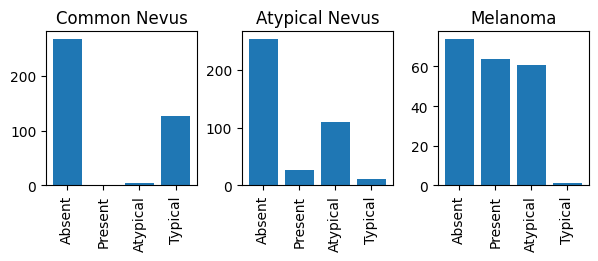
\includegraphics[scale=0.75]{images/ph2/ph2-dermo-diagnosis.png}
	\caption{Shows the labels of dermoscopic structures, number of images, and diagnosis. These are labelled between absent, atypical, present, and Typical.}
\end{figure}\label{ph2-dermo-diagnosis}

Figure\ref{ph2-dermo-diagnosis} shows dermoscopic structure labels relating to the diagnosis of the skin lesions. Common nevus have typical and present dermoscopic structures, atypical nevus have just as many absent with more present and atypical. Melanoma has more present and atypical types of skin lesions.

\begin{figure}
	\centering
	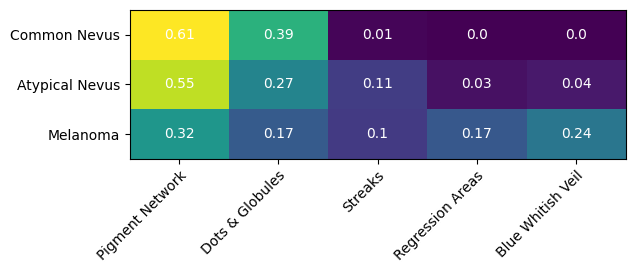
\includegraphics[scale=0.75]{images/ph2/ph2-diagnosis-dermo-heat.png}
	\caption{Shows the number of images based on the diagnosis and dermoscopic structures present, typical, and atypical.}
\end{figure}\label{ph2-diagnosis-dermo}

Figure\ref{ph2-diagnosis-dermo} demonstrates that pigment networks are present in both nevus and melanoma. Furthermore, streaks, regression areas, and blue-whitish veils are more common in melanoma. Pigment networks and dots/globules use different labels of typical and atypical so it is understandable they do not change between lesion types.

\begin{figure}
	\centering
	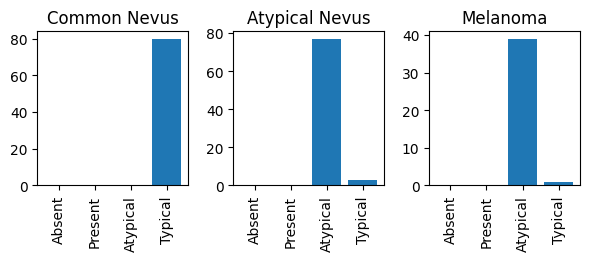
\includegraphics[scale=0.75]{images/ph2/ph2-pigment-diagnosis.png}
	\caption{Pigment network data relating to the diagnosis.}
\end{figure}\label{ph2-number-diagnosis-dermo}

There is little to no overlap between typical and atypical pigment networks between melanoma and naevus. Shown in figure\ref{ph2-number-diagnosis-dermo} common naevus are all typical pigment networks, while atypical naevus and melanoma are labelled atypical. This demonstrates that testing for pigment networks should be on type (typical and atypical) instead of whether they are present. Unusually, there is very little overlapping in the data. This is very unusual unless it was designed this way purposely, but it would have been more useful to have more samples without pigment networks.

\subsection{Diagnosis and Image Assessment}
%Show some of the asymmetry techniques that have been measured wrong, some seem to have been measured by colour and others only by shape. Consider excluding some.

Some of the images in the PH2 dataset have been organised regarding asymmetry through different means. For example, in figure\ref{ph2-image-assessment} one image is asymmetrical by colour, and another by shape. The assessments appear to be subjective, which is nothing new regarding ABCD rules, but considering they are from the same dataset it would be useful if they follow an objective measurement. Some written context would also have been massively beneficial.

\begin{figure}
	\centering
	%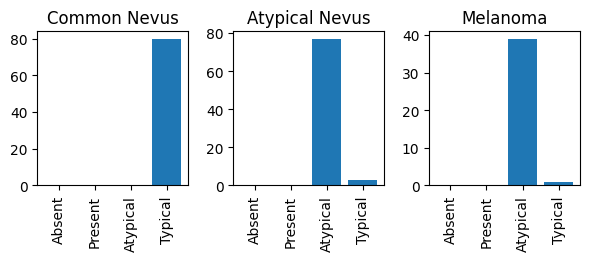
\includegraphics[scale=0.75]{images/ph2/ph2-pigment-diagnosis.png}
	\caption{}
\end{figure}\label{ph2-image-assessment}
b
%Show that the image assessment of some images is wrong, this was shown for asymmetry colour and shape

\subsubsection{Summary}
In summary, the PH2 dataset is a valuable resource for researchers considering it is the only one of its kind to provide metadata relating to asymmetry, colour, and dermoscopic structures. This has been used frequently in various studies to develop and evaluate algorithms for skin lesion analysis. Such datasets with substantial metadata are useful for producing explainable results. As explainable (XAI) becomes more common datasets describing clinical features will be necessary. However, one of the downfalls of this dataset is the unusual labelling for dermoscopic structures where the pigment network and globules are labelled between typical and atypical and others are between present and absent. Some metadata was inconsistent with the literature including the colour red, which is more common for melanoma, but the data does not demonstrate this. Furthermore, almost every image sample has a pigment network (although common), it would be more useful to have some without this feature.

An issue with this dataset is that many of the papers that utilise ABCD rules and dermoscopic structures do not test their algorithms against this dataset, regardless of the dataset being around before the time of publication\cite{Kasmi2016, She2007, Tenenhaus2010, Ramezani2014, Zaqout2016}. Instead they tend to use privately annotated datasets, which makes it difficult to replicate results. After analysing PH2 dataset it is likely the small size, lack of red colour samples and the unusual labelling of dermoscopic structures are the reason for this dataset being avoided. Furthermore, the ABCD rules tend to be subjective and are only relevant to the institution in which they are used, therefore this is likely again why the technique is being avoided and why many papers tend to annotate their data. Hopefully, some time in the future objective measurements can be accepted and datasets including vast data like PH2 will be accepted.

\section{Conclusion}
Overall both the PH2 and ISIC 2019 provide adequate data for the testing and developing algorithms. ISIC 2019 is suitable for training deep learning algorithms with a total sample size of 33,569 images with relevant metadata. PH2 is certainty the weakest link with data samples of only 200 images between benign naevi and moles and many papers refuse to test using the dataset and resort to privately annotating their
own data. Regardless PH2 appears to be suitable for analysis apart from the lack of red samples.

Considering the data distribution of the dataset both samples appear to be consistent with the literature. For example, in ISIC 2017 dermoscopic structures, SK has more samples with milia-like cysts and less pigment networks. Furthermore, melanoma and benign naevi have roughly equal pigment networks and less milia-like cysts. Another example is the colour distribution in PH2 while brown and light brown are common in benign neavi, MM has less samples of light and dark brown with more colours of blue, black, and white. The only sample that appeared to be wrong was the colour red, where there was a severe lack of samples.

\section{Developing the NHS dataset}
Whilst recognising the benefits of the ISIC 2019 and PH2 datasets we can begin to develop `the dataset' using NHS data. The inclusion of NHS data brings real-world clinical cases into the mix, and techniques developed during this project can be tested in the scenario it is intended to be utilised.

Requirements are decided below to highlight potential biases and issues, and then 2,000 images are chosen to create the dataset. This is followed by an analysis similar to the previous datasets and interesting findings from the data.

\subsection{Requirements}
%Describe the requirements, such as using macroscopic images over dermoscopic.
The use of machine learning algorithms for the detection of melanoma is a promising and evolving field with detection accuracies often beating that of dermotologists\cite{Andre2017}. However, the effectiveness of such depends heavily on the quality of the datasets used to develop them\cite{Tae2019}. The goal of this section is to describe and document the data extraction process from the National Health Service (NHS) and highlight biases, pre-processing, and other potential issues involved in the training of machine learning algorithms for the detection of melanoma. Requirements are first highlighted before gathering the data and are listed below.

There are requirements for this project, which include the use of macroscopic images instead of dermoscopic images. Macroscopic is described as viewing with the naked eye or by taking a picture with standard lenses. When referring to Dermoscopic images, are images captured with a specialised tool called a dermoscope that removes lighting variegation and improves the visual features within the skin lesion usually called dermoscopic features.

Although macroscopic images are used it is important to note that dermoscopy improves the diagnostic accuracy of dermatologists for melanoma when compared with macroscopic examination\cite{Wolner2017} and is widely considered superior\cite{Thiers2009}. Dermoscopic images provide a detailed visualization of patterns and structures on the surface of the skin lesion that might not be visible to the naked eye\cite{Thiers2009}. Some of these structures are pigment networks, asymmetry, irregular borders, and other features that support the differentiation between benign and malignant lesions\cite{Thiers2009}.

Another example shows the diagnosis for BCC was 91\% when using dermoscopy, compared to 57\% when using close-up images\cite{Dascalu2022}. Similarly, the sensitivity for SCC was 77\% with dermoscopy, compared to 70\% with close-up images\cite{Dascalu2022}. These findings highlight the superior diagnostic performance of dermoscopy compared to macroscopic.

The dermoscopic examination is superior to macroscopic examination, however, the project use case specifies macroscopic. The logic behind this is that the tool is specifically designed for general practitioners who are unlikely to recognize dermoscopic features, so there is no need to supply them with dermoscopes. This appears to be consistent with an author's findings showing that 92\% of dermatologists correctly recognize at least four size-types of melanoma. In contrast, only 38\% of non-dermatologists were able to recognize the same number of melanomas\cite{Tae2019}. Therefore, `the dataset' is created with macroscopic images for examination.

Considering the use of macroscopic images there needs to be a more thorough clean-up of the data for it to be used effectively. This will include removing hair and specular reflections to improve classification accuracy. This chapter will discuss the data transformation of NHS macroscopic images, including augmentation techniques to remove lighting, hair and other anomalous data from the images. All of which will support improving the accuracy when classifying.

\subsection{Data Biases}
The use of datasets is fundamental to the development and evaluation of machine learning algorithms, and the accuracy and effectiveness heavily weigh on the quality of the data used. Biases can arise from data collection procedures and pre-processing techniques. Not considering possible biases greatly affects machine learning algorithms using them and their effectiveness. Furthermore, careful consideration is essential to ensure the accuracy and reliability of the conclusions proposed in this document. Failure to consider all these factors could result in skewered conclusions that could undermine the validity of findings. For these reasons, it is essential to carefully identify and evaluate data before using and testing it.

NHS datasets contain a wealth of information that can be utilised. However, some biases need consideration before creating a dataset. These biases include:

\begin{enumerate}
	\item The diagnostic procedure dismisses skin lesions without recognizably suspicious features and does not reach the phase that photographs were captured. As such, there is a lack of typical benign skin lesions within the dataset, and most have some undesirable features.
	\item Dermatologists and general practitioners have diagnosed the large majority of skin lesions which have varying accuracy depending on their experience. Images include metadata on the department and person capturing the image, so the doctors' experience can be measured.
	\item Dermatologists could diagnose during an in-person examination where patients can be asked questions in real-time and further tests can be made involving touch. Otherwise, dermatologists diagnose using previously saved images, which might be less accurate because they lack the insight that an in-person examination would provide.
	\item Some skin lesions within the dataset lack metadata including their diagnosis. Such image samples should be avoided.
	\item Diagnoses of skin lesions are written in plain text including question marks where there is some uncertainty and the possibility of multiple diagnoses. Only diagnoses that are certain of their findings are used.
	\item Photographs of the skin lesions may be captured on different body parts such as hands, legs, face, and others. Most pre-processing methods are designed to differentiate between skin and skin lesions, so it is important to avoid using these images. Otherwise, new pre-processing methods will have to be made and tested.
	\item Seborrhoeic keratosis (SK) has similar features to that seen in malignant skin lesions. Therefore, there might be skin lesions diagnosed as melanoma that are SK. Furthermore, because of its similarity, there are many SK images. It will be vital to separate these.
\end{enumerate}

Following the potential issues 2,500 images were chosen from the NHS database. Eight types of skin lesions were chosen Malignant Melanoma (MM), Seborrhoeic keratosis (SK), Atypical Naevi (AN), Benign Naevi (BN), Squamous Cell Carcinoma (SCC), and Basal Cell Carcinoma (BCC).

%Go into more detail and graphs
\begin{enumerate}
	\item Malignant Melanoma (MM): A type of skin cancer that arises from melanocytes, which are responsible for the pigment melanin (brown skin).
	\item Seborrhoeic Keratosis (SK): A non-cancerous growth that originates from cells called keratinocytes.
	\item Atypical Naevi (AN): This refers to an unusual or atypical mole that shares characteristics of skin cancer, but they are not cancerous themselves
	\item Benign Naevi (BN): Normal benign mole that most people have.
	\item Squamous Cell Carcinoma (TM): A form of skin cancer that develops from squamous cells in the outer layer of skin.
	\item Basal Cell Carcinoma (BCC): The most common type of skin cancer, that develops from basal cells located in the outer layer of skin.
\end{enumerate}

The database system where the skin lesion images were located uses fotoware software. While there are a substantial number of images roughly reaching 20,000, these were obtained using diverse methods including dermoscopic and macroscopic. Other issues included and were removed:

\begin{enumerate}
	\item Dermoscopic (Not used in this study)
	\item Duplicates (keeping one)
	\item Skin lesions were not visible
	\item Abnormalities, edge of an ear or belly button
	\item Angled or far away images
	\item More than 2 skin lesions
	\item Almost entirely covered with hair
	\item Tattoo
	\item Scars
	\item Incision
\end{enumerate}

Some images were angled and far away which made it hard to get a clear view of the skin lesion. Others contained multiple skin lesions making it difficult to differentiate which one was being diagnosed. Others including tattoos and incisions were considered more extreme cases and deliberately excluded because there were not enough samples or outside the criteria of the project, respectively.

To remove the mentioned samples a search criteria was used, the example below is for finding melanoma:

\begin{center}
	("01 Close-up " -"Dermoscopy" -"eye lid" -ear -Nose -scalp -lip -cheek - scar -toe) AND (-SCC -BCC -"Seb k" melanoma -"atypical mole" -mole)
\end{center}

Some samples could not be removed automatically so they were removed manually by looking through the images. After finding all the samples, the following

\begin{enumerate}
	\item BN = 500 (600)
	\item AN = 500 (600)
	\item MM = 400 (500)
	\item SK = 200 (264)
	\item BCC = 200 (300)
	\item SCC = 200 (203)
\end{enumerate}

A significant difference between this and other datasets is the inclusion of benign naevi and atypical naevi. An atypical mole is an unusual naevi that has features similar to cancer but is non-cancerous. This will provide further insight into their distinguishing characteristics and into the difficulty of diagnosing atypical naevi from other skin lesions.

In the next section, further analysis of the images using the metadata will be conducted to remove image samples with uncertain diagnoses and to balance the dataset for better use with machine learning algorithms.

\section{Data Transformation and Analysis}
%Considering the data biases described in the previous section we can begin to piece together criteria that describe which images are appropriate for the creation of `the dataset'. Firstly, the most glaring problems are the diagnoses, because some images are missing diagnostic data and some have a variety of diagnoses, the scenario in which the diagnoses were captured is not mentioned, SK is potentially misdiagnosed as malignant, and the dermatologist that originally diagnosed is not mentioned. There are many ways to combat this problem. For example, during the creation of the PH2 dataset\cite{mendonca2013}, several dermatologists were asked to diagnose a skin lesion with appropriate metadata relating to the ABCD rules. If most dermatologists agree it is included in the study, otherwise it is removed. The goal of this is to minimize the incorrect data within the dataset. Alternatively, you might argue that removing less adequate records fails to prove whether the developed algorithms work in a real medical environment. Therefore, other methods were explored to validate the data.
%Very Unlikely we'll be getting histopathology data

%In this project, we do not have the resources to re-diagnose skin lesions, so instead the focus is on gathering diagnostic results from the histopathology department. These results are more accurate than dermatologists\cite{Morton1998} and counter the mentioned biases. Comparing this data with the diagnoses from the dermatology department provides insight into dermatology accuracy. Furthermore, histopathology serves as a ground truth for training the algorithms and testing their capabilities.

Each image holds metadata shown in table \ref{nhs-metadata} as EXIF Tags within each image. After extracting the images the metadata included in the images are Filename, Tags (Capturing method, anatomical location), Gender, DOB, Department, Consent, Historical Diagnosis, Diagnosis, and Date Photographed. There was other metadata with each image, but they are potentially identifiable, so to protect patient confidentiality, they were removed.

%Go into more detail and graphs
\begin{table}
	\small
	\begin{tabular}{|c|p{0.8\linewidth}|}
		\hline
		Attribute      & Description
		\\
		\hline
		Image ID       & an integer representing the image ID - example: 123456.xxx
		\\
		\hline
		\rowcolor{Red}
		Doctor         & a string representing the forename and surname of the doctor that made the diagnosis - example: JOHN SMITH
		\\
		\hline
		\rowcolor{Red}
		Department     & a string representing the name of the department - example: DERMATOLOGY
		\\
		\hline
		\rowcolor{Red}
		Studio         & a string representing the name of the studio used to capture an image of the skin lesion
		\\
		\hline
		Capture date   & an integer representing the date the image was captured - example: 00:00:0000
		\\
		\hline
		\rowcolor{Red}
		Hospital ID    & a string representing the hospital ID
		\\
		\hline
		Gender         & a string representing patient gender
		\\
		\hline
		Date of Birth  & an integer representing patient date of birth - example: 00-00-0000
		\\
		\hline
		\rowcolor{Red}
		Surname        & a string representing patient surname
		\\
		\hline
		\rowcolor{Red}
		Forename       & a string representing patient forename
		\\
		\hline
		\rowcolor{Red}
		Initials       & a string representing patient initials
		\\
		\hline
		\rowcolor{Red}
		Patient ID     & an integer representing patient ID
		\\
		\hline
		Subject (Tags) & an array representing method the image capturing method (Dermo or Close-Up) and anatomical location
		\\
		\hline
		\rowcolor{Red}
		Creator        & a string representing the forename and surname of the photographer - example: JOHN SMITH
		\\
		\hline
	\end{tabular}
	\caption{This table shows the metadata in each image and a description of each label. Rows highlighted in red are removed to protect patient confidentiality.}
\end{table}\label{nhs-metadata}

This is a generalised diagnosis, alongside these images are historical diagnoses of the skin lesion, written in plain text in some cases this question marks when the doctor is uncertain of a diagnosis and other times it includes a slash and a different diagnosis. Although it is not a specific format making it difficult to process, it includes a wealth of knowledge.

\subsection{Historical Diagnosis of Skin lesions}
The historical diagnosis is written text by the doctor that includes the possible diagnosis. The format is dependent on the doctor, so it changes dramatically. Generally, this is a `?' to show uncertainty and a `/' followed by another diagnosis. All of the variations in the format are shown in table\ref{nhs-naming}.

%Go into more detail and graphs
\begin{table}
	\centering
	\begin{tabular}{|c|c|}
		\hline
		Image ID    & Historical Diagnosis
		\\
		\hline
		998444.jpg  & SEB K
		\\
		\hline
		549982.JPG  & AK / SCC
		\\
		\hline
		824466.jpg  & ATYPICAL MOLE / ? MM
		\\
		\hline
		879067.jpg  & ? ATYPICAL NAEVI
		\\
		\hline
		1028628.jpg & ? MM / ? BCC
		\\
		\hline
		154414.jpg  & 1) ? SCC 2) SBCC 3) ? SPOT
		\\
		\hline
		739199.JPG  & (1) BOWEN'S DISEASE (2) SUPERFICIAL BCC
		\\
		\hline
		586010.JPG  & SUSPECTED N. MM
		\\
		\hline
	\end{tabular}
	\caption{Examples of historical diagnosis and doctors and some unique variations of labelling.}
\end{table}\label{nhs-naming}



\begin{figure}
	\centering
	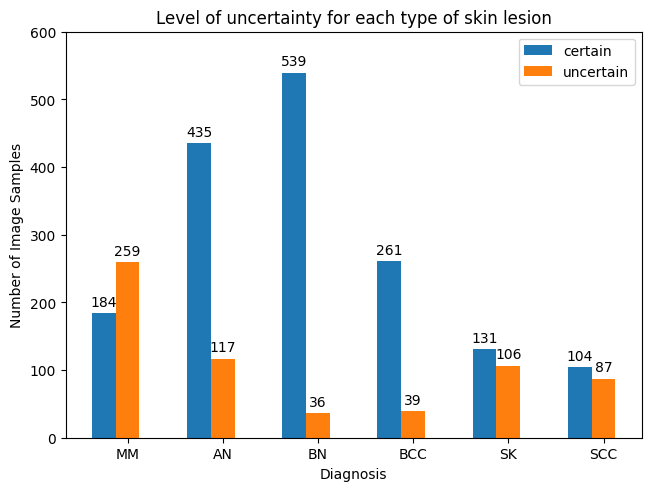
\includegraphics[scale=0.75]{images/nhs/nhs-diagnosis-certainty.png}
	\caption{Number of image samples relating to the historical diagnosis. Labelled as uncertain if there is a `?' in the diagnosis.}
\end{figure}\label{nhs-diagnosis-certainty}

Some historical diagnoses contain a `?' showing uncertainty from the doctor. Figure\ref{nhs-diagnosis-certainty} describes the number of skin lesions between uncertain and certain. Interestingly AN, BN, and BCC appear to be certain with 117, 36, and 39 respectively. Followed by SK and SCC are roughly half of the images at 106 and 87. Most of all MM shows that more than half of the diagnoses at 259 are uncertain out of 184 that are certain. This in turn demonstrates the type of skin lesions that doctors are having difficulty diagnosing where melanoma is especially difficult.

\begin{figure}
	\centering
	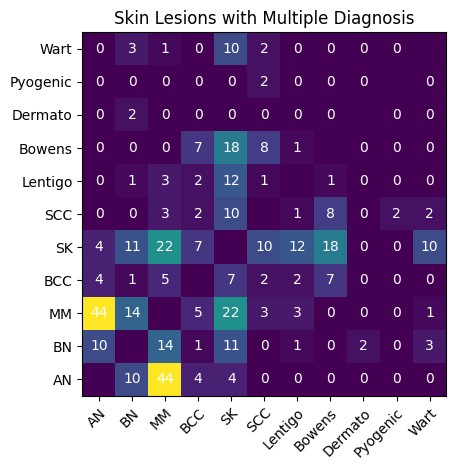
\includegraphics[scale=0.75]{images/nhs/nhs-multiple-diagnosis.png}
	\caption{Number of skin lesion samples with multiple diagnoses in the historical diagnoses. Other types including lentigo, Bowen's disease, dermatofibroma, pyogenic granuloma, and wart are only associated with the main diagnoses (AN, BN, MM, SCC, BCC) because they are not specifically searched for. This means they are only found in association with the mentioned main diagnoses and this data is likely missing data comparing the other types.}
\end{figure}\label{nhs-multiple-diagnosis}

Multiple diagnoses are sometimes shown, figure\ref{nhs-multiple-diagnosis} shows the number of skin lesions with multiple diagnoses mentioned in the historical diagnoses. Interestingly the most commonly associated are AN with MM at 44 and SK with MM at 22 images. Others are SK with MM, Bowen's disease, lentigo, warts, and SCC demonstrating that SK is associated with the widest range of skin lesions and the difficulty diagnosing it.

\begin{figure}
	\centering
	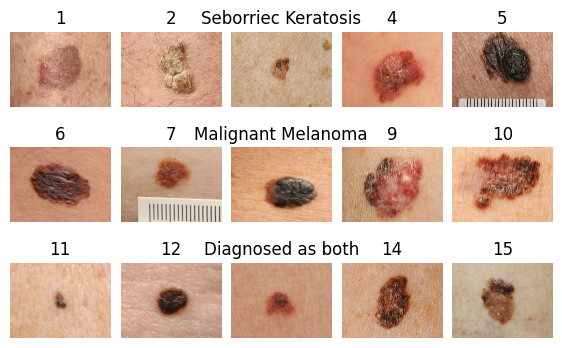
\includegraphics[scale=0.75]{images/nhs/nhs-mm-sk-examples.png}
	\caption{Comparing skin lesions that are diagnosed as MM, SK, and considered both MM and SK.}
\end{figure}\label{nhs-mm-sk-examples}

Considering that SK has multiple diagnoses mostly for MM and SK, it is a good idea to compare these images and see whether there are any distinguishing features. Demonstrated in figure\ref{nhs-mm-sk-examples} SK border and colours change dramatically between different lesions demonstrating how difficult it is telling them apart\cite{}. The ABCD rules and TDS is assigned to each image to see whether this diagnostic procedure will be suitable for separating these skin lesions.

\subsection{Anatomical location}

%Data extraction Techniques
Anatomical location has a total of 28 different descriptors for specific body parts including leg, wrist, neck, etc. To make comparisons easier with the ISIC dataset each label has been assigned to specific areas such as upper extremity, anterior torso, etc. All the locations are listed in the table\ref{nhs-location-names}.

%Go into more detail and graphs

\begin{table}
	\centering
	\begin{tabular}{|c|c|}
		\hline
		Category        & Organised sub-labels
		\\
		\hline
		Upper Extremity & Wrist, Elbow, Arm
		\\
		\hline
		Lower Extremity & Leg, Knee, Hip, Ankle
		\\
		\hline
		Lateral Torso   & Axilla, Breast
		\\
		\hline
		Posterior Torso & Back, Shoulder
		\\
		\hline
		Anterior Torso  & Chest, Abdomen, Trunk
		\\
		\hline
		Palms/Soles     & Hand, Thumb, Foot
		\\
		\hline
		Oral/Genital    & Groin, Genitalia, Sacrum, Buttocks, Sacrum
		\\
		\hline
		Head/Neck       & Neck, Chin, Face, Temple, Head, Forehead
		\\
		\hline
	\end{tabular}
	\caption{All the different labelling for the anatomical location of the lesion. Each label in the NHS data has been assigned to a category similar to the ISIC dataset.}
\end{table}\label{nhs-location-names}

%Show transforming the images into the correct size

\section{Data Transformation and Augmentation}
As mentioned in the data biases section the skin lesion images are taken under various conditions including angles, lighting, and distance from the skin lesion. While the variety of conditions will decrease the accuracy of results and hinder the detection of dermoscopic features, it is a requirement of the project.

One of the main challenges in melanoma detection is the visual similarity between normal and infected regions. Others are the presence of artefacts such as bubbles, hair and clinical marks\cite{Albahli2020}. These factors lead to low accuracy rates in traditional approaches. However, segmentation techniques can help overcome these challenges by removing these areas and isolating the melanoma from the rest of the image.

Skin lesion augmentation is especially vital because of the use of macroscopic images instead of dermoscopic images. This means there are various artefacts including hair, specular reflections, rulers, varying sizes, and shapes of the skin lesion. All of these can obscure the skin lesion and affect the accuracy of segmentation\cite{Unver2019} and in effect feature detection.

By augmenting the skin lesion images using specular reflection removal and hair removal, the accuracy of feature classification methods can be improved\cite{kasmi2023}.

\subsection{Hair Removal}
Hair artefacts in images can interfere with the recognition of handcrafted features and affect the performance of deep learning algorithms in melanoma detection\cite{kasmi2023}. Applying morphological operations such as image sharpening and segmentation techniques can remove hair artefacts from dermoscopic images\cite{kasmi2023}.

Dull-Razor is an algorithm developed by Lee et al\cite{Lee1997} and is frequently implemented with

Sharp-Razor\cite{kasmi2023} is a technique for detecting hair and ruler marks to remove them from images. This uses a multiple-filter approach including grayscale plane modification, hair enhancement, segmentation using tri-directional gradients, and multiple filters for hair of varying widths. This technique is shown to outperform existing methods.

\subsection{Specular Removal}
Specular reflection removal techniques are effective in improving the accuracy of melanoma detection\cite{Shen2009}. A technique was proposed utilizing a partial differential equation to iteratively erode the specular component, removing the specular reflection\cite{Shen2009}.


\section{Conclusion}



\section{Dataset Statistics}
The dataset has been analysed and modified accordingly, originally starting with a total of 2,500 images and it has been amended to 2,271.

\begin{figure}
	\centering
	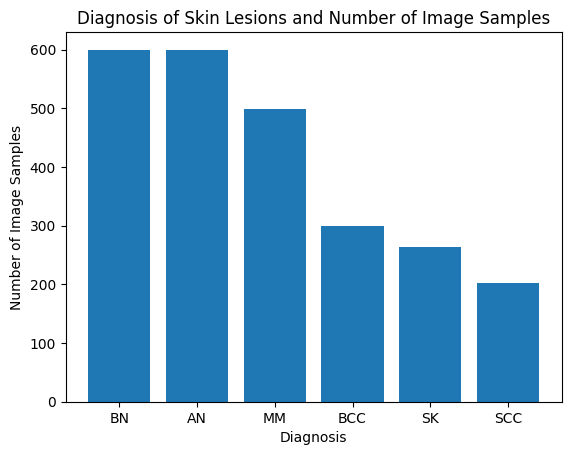
\includegraphics[scale=0.75]{images/nhs/nhs-diagnosis.png}
	\caption{Number of image samples relating to the diagnosis of the image.}
\end{figure}\label{nhs-diagnosis}

As shown in figure\ref{nhs-diagnosis} the image data and diagnosis of the skin lesion there are several differences in this dataset compared with the ones described so far. There has been more of an attempt to balance the data so there are more equal samples of each. Furthermore, benign naevi have been split into benign naevi (BN) and atypical naevi (AN). There are images of seborrheic keratosis, which is more than any other public dataset currently available.

\begin{figure}
	\centering
	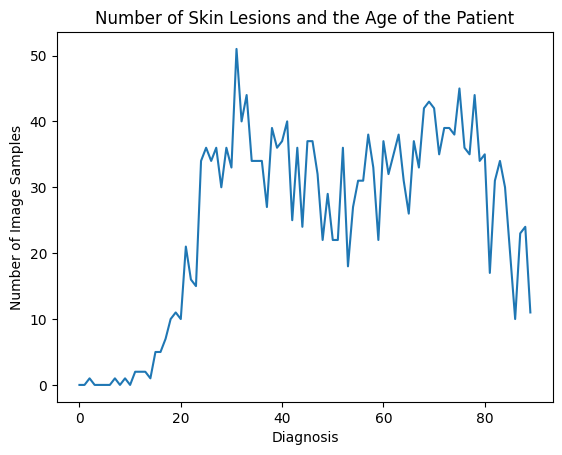
\includegraphics[scale=0.75]{images/nhs/nhs-age.png}
	\caption{Age of patients and number of image samples.}
\end{figure}\label{nhs-age}

The age variation of patients described in figure\ref{nhs-age} demonstrates there are many younger patients included in the NHS dataset. This is substantially different from other datasets including ISIC that have mostly older patients. This demonstrates that there is an influx of younger patients regardless of them not being within the age group where melanoma usually develops. In both ISIC and NHS datasets the median the median is 60 years.

\begin{figure}
	\centering
	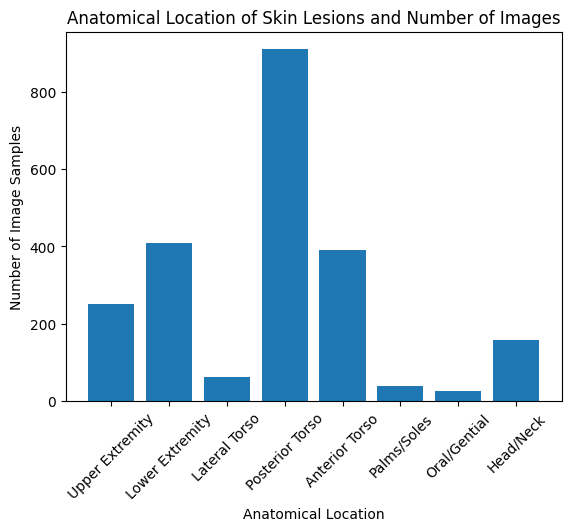
\includegraphics[scale=0.75]{images/nhs/nhs-location.png}
	\caption{Number of image samples related to the location of the skin lesion.}
\end{figure}\label{nhs-location}

As shown in figure\ref{nhs-location} describing the location of the skin lesions and several image samples. There are more samples on the posterior torso (back) compared with other skin lesions with any of the others. There are only a couple of samples for lateral, palms/soles, and oral/genital. This data was originally modified because it had a total of 28 descriptors, so they were grouped into 8 similar to the ISIC dataset. This can be seen in more detail in figure\ref{nhs-location-names}.

\begin{figure}
	\centering
	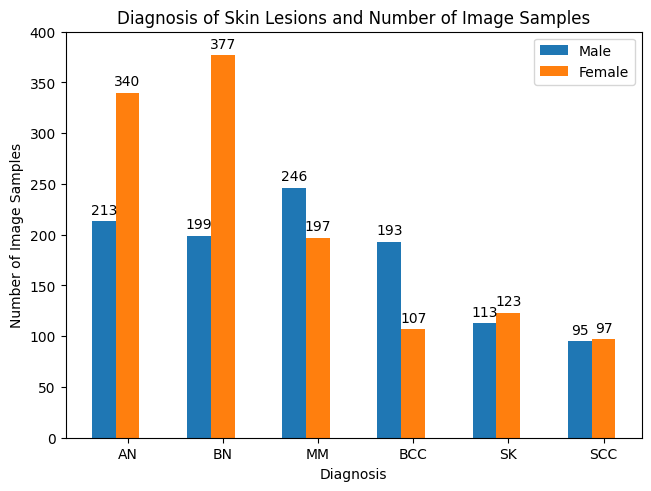
\includegraphics[scale=0.75]{images/nhs/nhs-sex-diagnosis.png}
	\caption{Number of image samples relating to the diagnosis and sex of the patients. There are more female than male patients.}
\end{figure}\label{nhs-sex-diagnosis}

Figure\ref{nhs-sex-diagnosis} describes the number of image samples relating to the diagnosis and sex of the patients. Interestingly there are almost double the number of female patients being diagnosed for AN and BN compared with MM where there are slightly more male patients and BCC where there is almost double male.

\begin{figure}
	\centering
	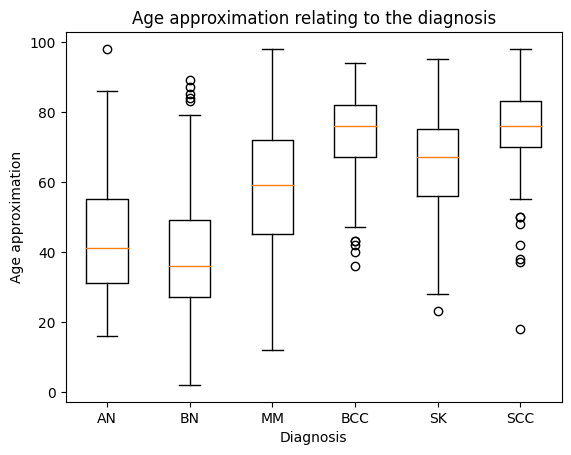
\includegraphics[scale=0.75]{images/nhs/nhs-diagnosis-age.png}
	\caption{Boxplot describing the age of patients and the diagnosis.}
\end{figure}\label{nhs-diagnosis-age}

Image samples described in figure\ref{nhs-diagnosis-age} demonstrate the age of patients compared with their diagnosis. Understandably, AN and BN which are neavus are from younger patients, while SK, SCC, and BCC appear in older adults. MM is primarily from patients at the age of 50 to 70.

\begin{figure}
	\centering
	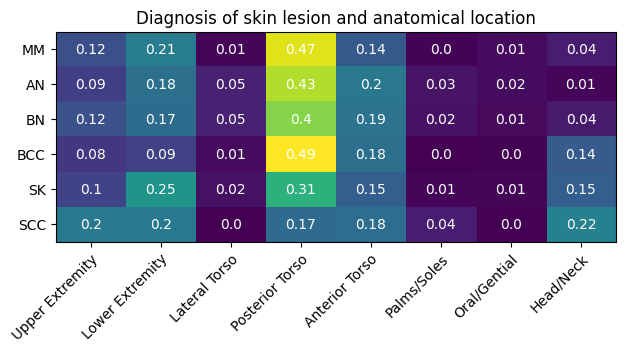
\includegraphics[scale=0.75]{images/nhs/nhs-location-diagnosis.png}
	\caption{Number of image samples relating to the diagnosis of the image.}
\end{figure}\label{nhs-location-diagnosis}

